\documentclass[12pt]{article}

%opening
\title{Malicious context and workaround analysis of decentralized VPN:\\the case of Mysterium Network}
\author{Jacopo Federici}


\usepackage{imakeidx}
\usepackage{setspace}
\usepackage{url}
\usepackage{graphicx}
\usepackage{listings}
\usepackage{array,multirow,graphicx}
\usepackage{float}
\usepackage{xcolor}
\usepackage{tcolorbox}

\lstset
{
    language=bash,
	basicstyle=\ttfamily,
    numbers=left,
    stepnumber=1,
    showstringspaces=false,
    tabsize=1,
    breaklines=true,
	breakatwhitespace=false
}

\newtcbox{\tag}{on line,
  colframe=lightgray,colback=lightgray,
  boxrule=0.5pt,arc=2pt,boxsep=0pt,left=2pt,right=2pt,top=1.5pt,bottom=1.5pt}

\makeindex

\begin{document}
	\raggedright
	\setstretch{1.0}
	\maketitle	
	\clearpage
	
	\tableofcontents{}
	\pagebreak

	\begin{abstract}
		
	\end{abstract}
	\pagebreak

	\subsection{Work structure}
	\subsection{Outline}
	\subsection{Goal}

	\section{Introduction}
	Privacy is increasingly becoming a central topic of discussion in many different fields, as the need to protect our data is becoming critical. The massive digitalization of many aspects of our life implicitly exposes us, and our data to possible attacks. Even the simplest operations over the internet are becoming unsafe.\\
	In the last years, we have seen security solutions integrated into popular applications, such as browsers or mobile apps, to prevent increasing attacks to users' security. For instance, in 2017, the popular browser Google Chrome, announced that it would have marked as non-secure any website using the HTTP protocol instead of HTTPS. The HTTPS protocol is the standard HTTP protocol that uses SSL/TLS certificates, an additional security layer to make the communication between clients and servers secure. Before that, connections were not protected by any encryption algorithm.\\
	Even though the first HTTPS protocol was proposed by Netscape Navigator b in 1990, it is only in more recent years that we started assisting to a global trend to increase security levels, often achieved BY encrypting communications.\\
	The Chrome browser initiative is part of a global trend to increase the security level, often achieved encrypting the communication: instant messages applications, internet protocols like the DNS, industrial system infrastructures, and many others.\\
	Although the level of security of the internet has substantially increased, there is still a wide range of situations and scenarios in which the individual user browsers the internet in an unsafe way.\\
	A solution to increase the security level is provided by the Virtual Private Network (VPN), a technical solution that allows extending a private network across a public network. It creates a virtual point-to-point connection by using a tunneling protocol over the existing network, and the tunneled traffic is encrypted. A first proposal of the VPN specification is around 2000 \cite{VPNRFC}, but only in the last years, the use of VPN became massive. The VPN data encryption feature is solving privacy problems of various nature, such as to exit a censored network, using services available or blocked in certain countries, avoiding tracking methods and other similar scenarios.\\
	Currently, there are commercial solutions that allow users to have a private connection to the company's servers across the world, but there are many security concerns about those solutions. These companies can keep the connection logs, inspect the traffic, or sell statistical data.\\
    Some open-source projects were, lately, born to solve these issues. Their goal is to revolutionize the idea of VPN and its uses, building a rich network of peers where two nodes can connect through a VPN. The projects provide a platform that includes all the components needed to have an efficient, fast, and easy-to-use system, from the discovery to the payment.\\
    
    In this research, we analyzed the most developed project, Mysterium Network, as a case of study. As we write, Mysterium offers a working network composed of hundreds of nodes around the world, making it the best project to investigate malicious contexts and to design vulnerabilities, owns by the decentralized architecture, more than the Mysterium project itself.\\
	We even discover how secondary aspects are pivotal to guide attacks to the system.\\
    Then we focus on the solutions that can patch those critical aspects and provide a comparison of them with an eye on the practical perspective.
	
	\subsection{The state of the art}
	The world is changing at a fast pace.\\
	First, everything is now much faster. The internet infrastructure allows us to move significant amounts of data in just a few seconds. Furthermore, our personal computer can perform operations that were impossible to execute some years ago on mainstream servers. This speed increases the computational power, and it is jeopardizing many security solutions, such as ciphers that based, and still base, their strength on the practical difficulties to solve the mathematical problems at the foundation of cipher methods.\\
	Second, the architecture is moving back to a cloud-based infrastructure. Many workflows see, again, a thin client sending the execution step to a cloud server that elaborates the output that is then sent back to the client. This architecture changes the surface of the attack targeting the cloud servers as the principal attack destination.\\
	Third, some technologies are mature enough to provide an excellent alternative to traditional models — for instance, the cryptocurrency model against the bank model. Here, the changes are in the paradigm, and the reasons behind these new approaches are much more than technological.\\

	\textit{The security noun is changing the meaning inside the people's minds, from "how thick is my bank caveau" to "how long my bank requires my new online account password"}

	\subsection{the need for trust and privacy}

	\begin{verbatim}
		https://www.geeksforgeeks.org/need-of-information-security/
		https://www.hackerfactor.com/blog/index.php?/archives/868-Deanonymizing-Tor-Circuits.html
		https://www.howtogeek.com/133680/htg-explains-what-is-a-vpn/
		https://www.forbes.com/sites/tjmccue/2019/06/20/why-use-a-vpn/#3f08d7105859
		https://www.investopedia.com/terms/b/blockchain.asp
		https://www.howtogeek.com/350322/what-is-ethereum-and-what-are-smart-contracts/
		
		https://en.wikipedia.org/wiki/Proof_of_work
		https://en.wikipedia.org/wiki/Proof_of_stake
	\end{verbatim}

	Technology is becoming an essential tool to exercise the people's rights. There are areas of the world where these rights are not accessible, and people fight to obtain them. For example, in the People's Republic of China, the government built a firewall to censure the internet. It is called the Great Firewall Of China, abbreviated in GFW, and it is a combination of laws and technologies to control the internal domestic internet, so-called censorship. It blocks social networks, search engines, and many other services that declined the government's request to make the traffic clear and detectable.\\
	In this context, aspects such as anonymization, become not only relevant but crucial to be preserved.\\
	As for anonymization, a solution to obtain identity obfuscation is the VPN. It is massively used to protect data from surveillance at any level, from a public unsecured wifi connection to the country Internet Service Providers.\\VPNs are provided by companies that often do not act genuinely, making the identity or the traffic detectable or, even worsts, sniffing and crafting the data for malicious actions.\\

	The decentralized VPN completely changes the paradigm, the design of the infrastructure.\\
	An analogy can be made with the traditional bank model: as we know, the bank is a centralized entity trusted by definition. What if the bank suddenly becomes untrusted? Cryptocurrencies spread among ourselves, the cryptocurrency owners and network participants, the trusts we put in the bank, using a blockchain as a technical solution. 
	A similar design is used with decentralized VPN: there is no central entity to control the system, but a significant number of peers, the network, we can choose to connect.

	\subsection{Decentralized systems}

	\subsubsection{dVPNs}

	A decentralized VPN is a network of nodes where the users can connect through a VPN to nodes without a central entity. It allows the user to create a private tunnel with another user, making encrypted all the traffic between the two points. 
	The decentralization system, in this context, includes several steps to make the final connection happening, rather than a simple VPN connection between two peers.\\
	First of all, the user creates an identity into the system, linked to the payment wallet, using a client application. Then, he connects to the network providing his availability to be a consumer or a provider.\\
	The consumer user chooses the provider he prefers based on different features such as the region, quality, or cost of the node, and asks for a new connection to that server. In this step, the blockchain, based on Ethereum, allows creating a smart contract between the two participants with a predetermined amount of money. Using commercial VPN applications, such as OpenVPN or Wireguard, the connection between consumer and provider, otherwise called client and server, is established. When the connection correctly ends, the network closes the smart contract, that registers the result of the transaction in the blockchain.\\
	We outlined the main steps from which we can think of a decentralized VPN more as a platform solution rather than a simple VPN application. Indeed, other projects suggested the VPN is one of the features a decentralized system so composed can have. (EXPLAIN BETTER THE IDEA)  
		          
	\subsubsection{The business idea}
	As a business project, which aims to earn money, the project has a specific business plan: provide a system network where users can join as a service provider, selling their internet bandwidth, or as a service consumer, buying other's internet bandwidth. For every cryptocurrency transaction, the network applies a fee that wants, substantially, to create a market to manage.\\
	Each couple of entities, a consumer and a provider, agree on a transaction paid using cryptocurrency in the face of the used service. This transaction is regulated by an Ethereum smart contract signed by both sides and requires a fee to be closed. This fee is not the Ethereum fee, generally called gas, but the precisely Mysterium source of earnings. For this reason, Mysterium and other projects created their coins used to buy and sell internet bandwidth between the nodes inside the network. The coin name is MYST for Mysterium Network and, as a regular cryptocurrency, it is possible to convert MYST to ETH and vice versa.\\
	Although a node can decide to be a consumer or a provider at any moment, the two entities are different, and the type of market is called a two-sided market where bid and ask respectively grow on the other side growth. (EXPLAIN BETTER)\\

	(BID AND ASK GRAPHIC DEPENDING ON THE FEES)

	\begin{verbatim}
		concetti introduttivi
		- blockchain in linea di massima\\
		- ethereum in linea di massima e descrizione degli smart contracts\\
		- proof of work, proof of stake\\
		- reputazione in una net (Eigentrust)\\
		- - cercare applicazione pratica di Eigentrust\\
		- descrizione di BFT\\
	\end{verbatim}
	
	\section{Mysterium Network}
	
	The main open-source projects which aim to create a decentralized VPN are Mysterium Network, Privatix, Substratum, and Sentinel. We explored all of them, and we can safely say the most advanced project is Mysterium Network, at the time we are writing this research.\\It is the most completed in terms of development and design. Furthermore, it's 100\% open source, that for this kind of project is a requirement which conditions the users' adoption and the market diffusion.\\
	Therefore, we decided to use the Mysterium Network as a test case to analyze the malicious context the project is exposed to and propose our proof of concepts as solutions.
	
	\subsection{Architecture}
	Mysterium Network is an open-source project. Its main goal is to build a decentralized infrastructure made up of layered VPN protocols, blockchain, and smart contracts.\\
	As described in figure X, we can distinguish between a service client block and a service provider block. Both of them lean on the Ethereum blockchain block, which is a distributed database where all the network operations, the identities, and the service proposals are recorder.\\

	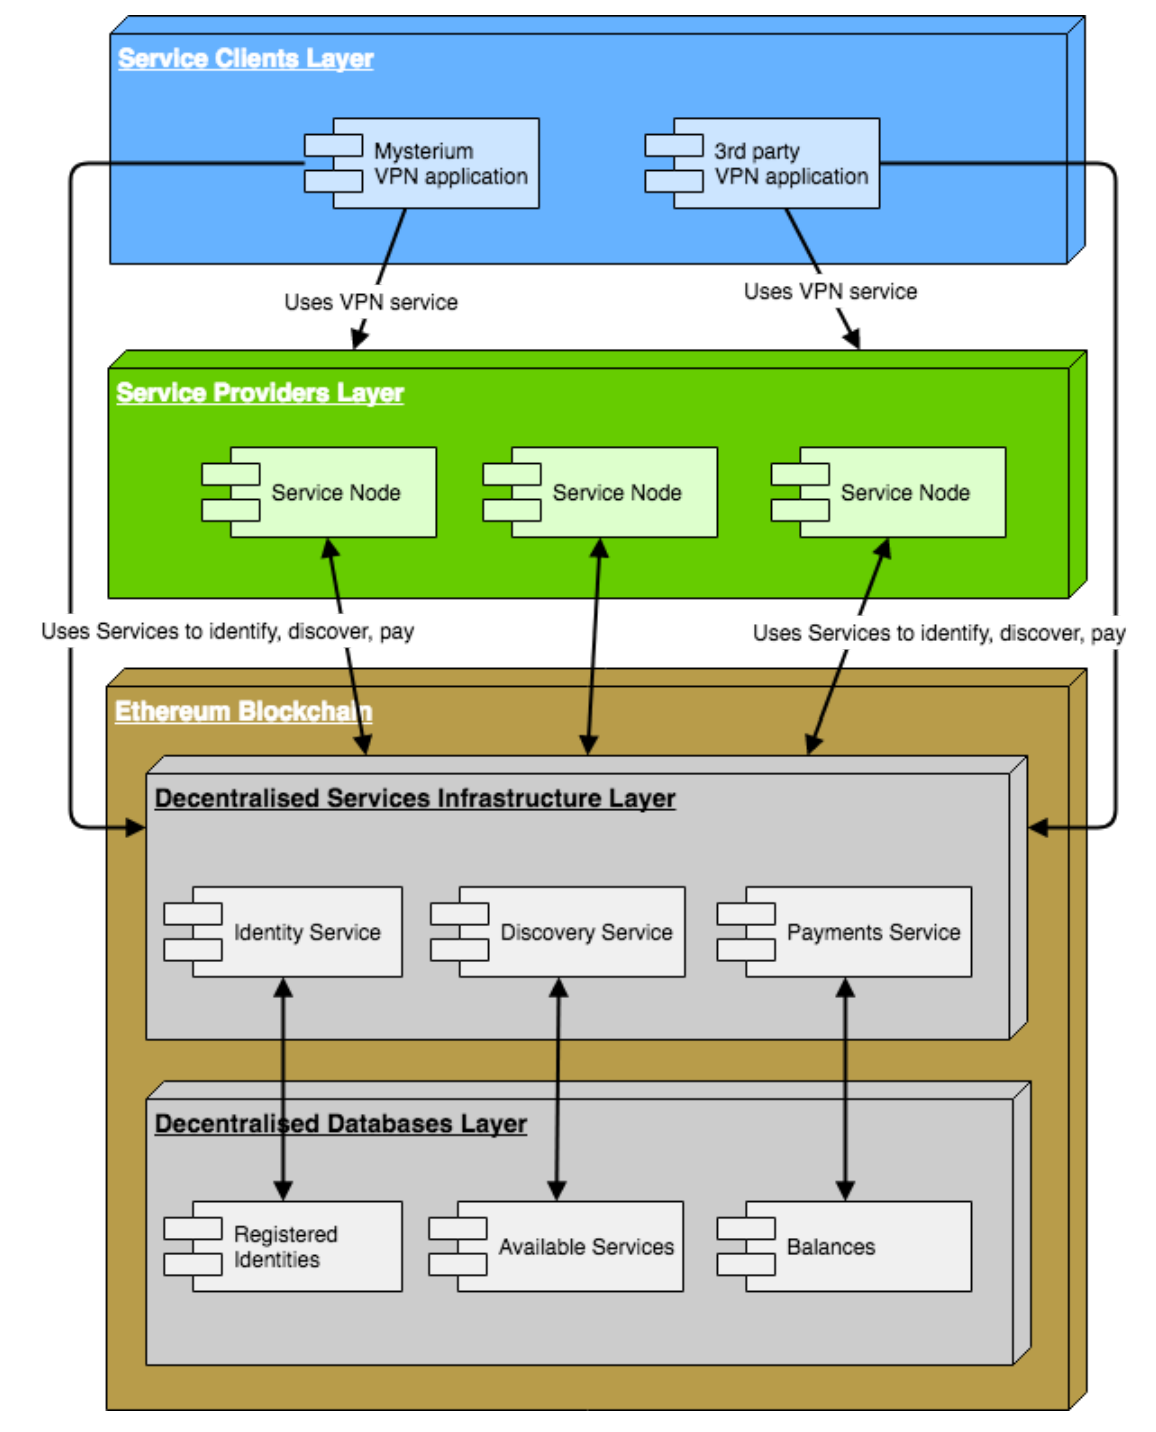
\includegraphics[width=0.5\linewidth]{images/mysterium_architecture.png}
		
	As a general workflow description, Mysterium starts by collecting all the agents' service proposals and presents them to the clients. Then it registers the client's intention to pay for the agent's service chosen by the user and creates the VPN connection between the two points. The outcome of each transaction is saved in the blockchain.\\
	
	To implement all the functionalities just said, Mysterium has four core components inside its architecture:
	\begin{itemize}
		\item \textbf{Ethereum Blockchain} allows running decentralized code with smart contracts, enabling reliable services and payment handling.
		\item \textbf{Identity service and database of registered identities} ensure the proper identity acknowledgment between client and service provider.
		\item \textbf{Discovery service and database of available services} provide means to announce the availability of VPN services and to pick the most suitable VPN service.
		\item \textbf{Payment service and database of balances} allow secure promise-based micropayments for services.
	\end{itemize}

	\subsubsection{Identity Service}

	The \textbf{identity service} manages the network identities that every node needs. A single node can create one identity or more, and each of them consists of a public and a private key. The last 20 bytes of the hash function, applied on the public key, is the unique id used to identify the node into the network. To publish a new identity so that other network members can reach it, Mysterium uses the smart contract mechanism. The private and public keys are used to validate the signature for the communication between the nodes.\\
	The blockchain mining process appends the public key and the unique id to the Ethereum blockchain after the node pays a fee to the network. This amount of money has the purpose of giving value to the identity. In such a way,  to abandon the identity to create a new one is unattractive, because it is expensive, but not impossible.\\ 
	We will discuss those aspects later, but we can surely say this is the first barrier to block in mass identity creation.\\
	Furthermore, the user benefits in using the same identity because it is possible to rebuild his transaction history and his balance from the Ethereum blockchain, making the user more predictable and thus trustworthy for service providers.\\

	\begin{figure}
		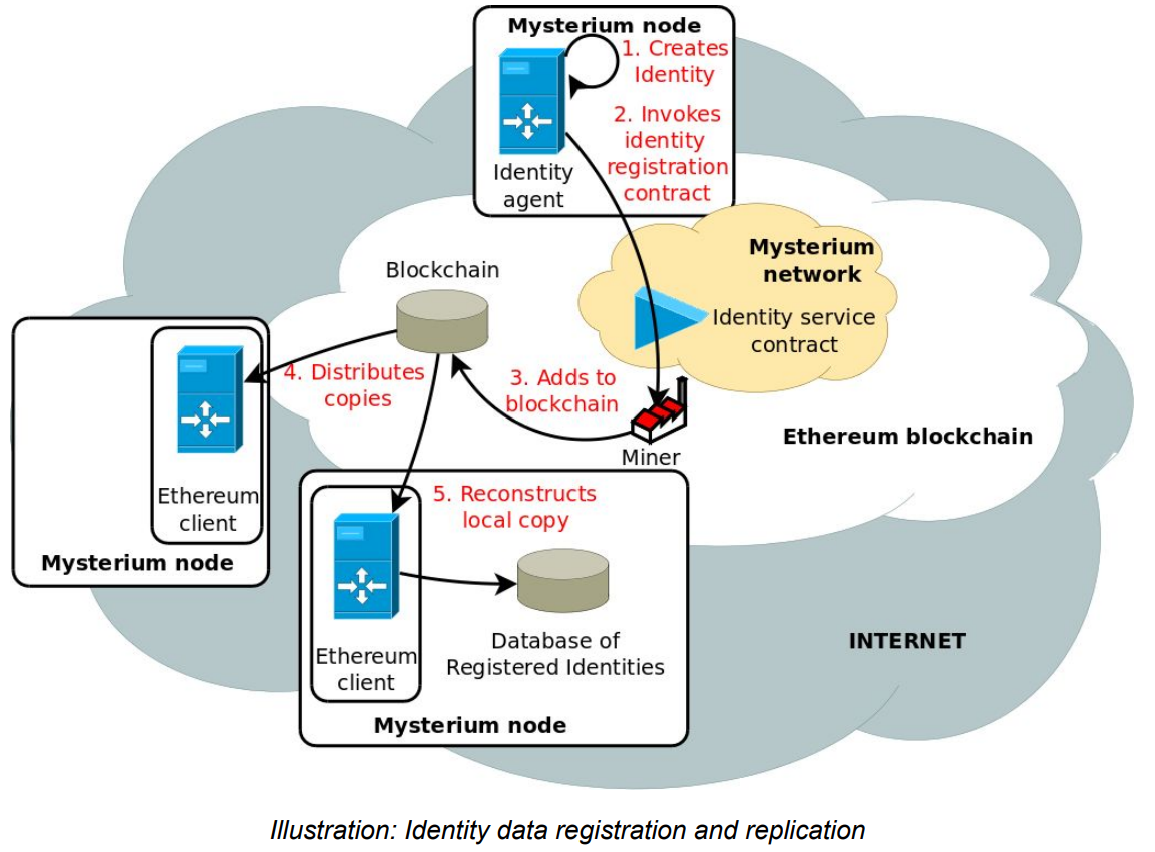
\includegraphics[width=0.5\linewidth]{images/mysterium_identity_creation.png}
		\caption{The Mysterium identity creation steps}
	\end{figure}

	\subsubsection{Service Discovery}

	The \textbf{service discovery} provides the list of service proposals available in the network. The service posts its service offer characterized by some service parameters: those parameters can be the VPN application the provider supports, the provider's connection IP address and port, the provider's server location, or the bandwidth per session. Then, the miners append the proposal to the blockchain, making it publicly available for everyone.\\

	\begin{figure}
		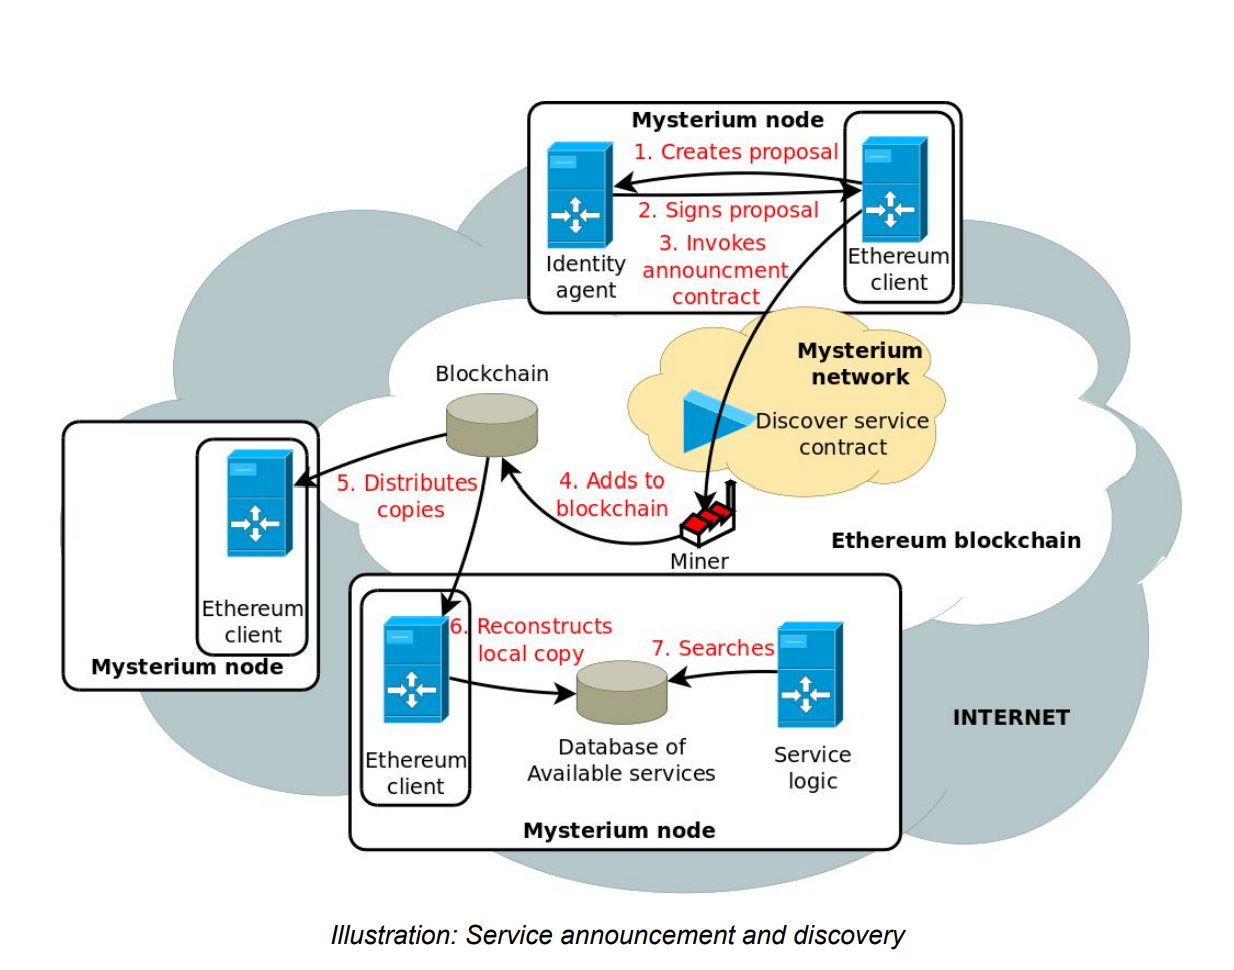
\includegraphics[width=0.5\linewidth]{images/mysterium_service_announcement.png}
		\caption{The Mysterium service announcement steps}
	\end{figure}
	
	\subsubsection{Payments Handling}

	Ethereum blockchain holds all the mechanisms for the \textbf{payments handling}. Therefore everyone needs an account to operate in the Mysterium Network. To advance a request, the consumer has to deposit currency in his wallet. Then, he can ask for a connection to a provider who has previously published a service proposal. Mysterium describes this step as a promise creation because the client effectively promises he will pay when the service ends. Positively clearing a promise is the everybody's best interest, the producer and the consumer, since a canceled promise marks the consumer's history hitting his reputation for future connections.\\
	From what we have described so far, it seems the consumer can decide to avoid paying for the used service: technically, it is possible, but realistically there are some considerations to be made.\\
	First of all, as previously described, identity creation takes money to be completed, and for any new connection, the user's balance has to be positive. In any case, the blockchain records any connection result so that everybody can rebuild the user's history at any moment. Therefore, it is possible to deduct the user's reputation based on its history.\\
	Using this reputation, the provider can decide to block his service to all users that have a low reputation caused by an unpaid precedent. On the other hand, other providers allow new users' connections with a low reputation but at a high price, accepting the risk of having an unpaid transaction.\\
	
	\subsection{Components}

	The core application is called \textbf{node}. It's written in GoLang, a new program language made by Google that is having a high adoption in the last years. The node creates a local webserver to connect to the network, manages the cryptocurrency wallet, and initiates the VPN connection as a client or manages the incoming connection as a server. Mysterium leans on famous VPN applications, which are OpenVPN and Wireguard.\\
	The node can be run in two modes, as a client or as a server, and it is managed via command-line interface or RESTful API, called TequilaAPI, exposed in the localhost.\\
	The main functionalities of TequilaAPI concern:
	\begin{itemize}
		\item the authentication,
		\item the connection,
		\item the identities,
		\item the location,
		\item the proposals,
		\item the service operations in provider mode
		\item other minor features
	\end{itemize}

	TequilaAPI is used by the client's application to manage the connection and for diagnostic operations.\\
	Mysterium developed a desktop client written using Electron, which uses the TequilaAPIs.\\
	The node is also available as a ready-to-use Docker image and published on the Docker Hub.\\
	On the mobile side, Mysterium is present with its multiplatform app that works only as a client.\\
	(MORE ON MOBILE)

	\subsubsection{Technical description}

	We have chosen the Linux platform and OpenVPN as the VPN application, but similar considerations can be made with different configurations.\\
	When the Mysterium application starts, it calls OpenVPN, which sets up its network environment. OpenVPN creates a virtual network device used to encrypt and decrypt the traffic. These devices reside in the kernel and are entirely virtual, which means there is no hardware on their back.\\
	They can be of two types, TAP or TUN.\\
	The TAP type is used to simulate a link layer device, which means the corresponding ISO model level it refers to is number two. Therefore, a TAP interface handles the transmission of the data frames between two nodes on the same physical layer. The behavior is equal to a bridge device: to connect two separates networks as if they were one.\\
	On the other hand, the TUN type is, in the ISO model, one layer above, working at level three. A TUN interface handles packets, such as Internet Protocol packets. The main functions include port forwarding, host addressing, and traffic control, for example. The behavior is, in this case, equal to a router device: to connect two separates networks allowing their communication but keeping them independent.\\
	Usually, the TUN type is the most used, since the TAP type brings some limitations such as it cannot be used with Android or iOS devices, causes higher overhead on the VPN tunnel, and scales poorly.\\
	The following schema describes an example of a scenario where the network has two ethernet cards, one public and one internal.\\
	The virtual TUN interface created by OpenVPN is tun0, the public interface is eth0, and the internal interface is eth1.\\

	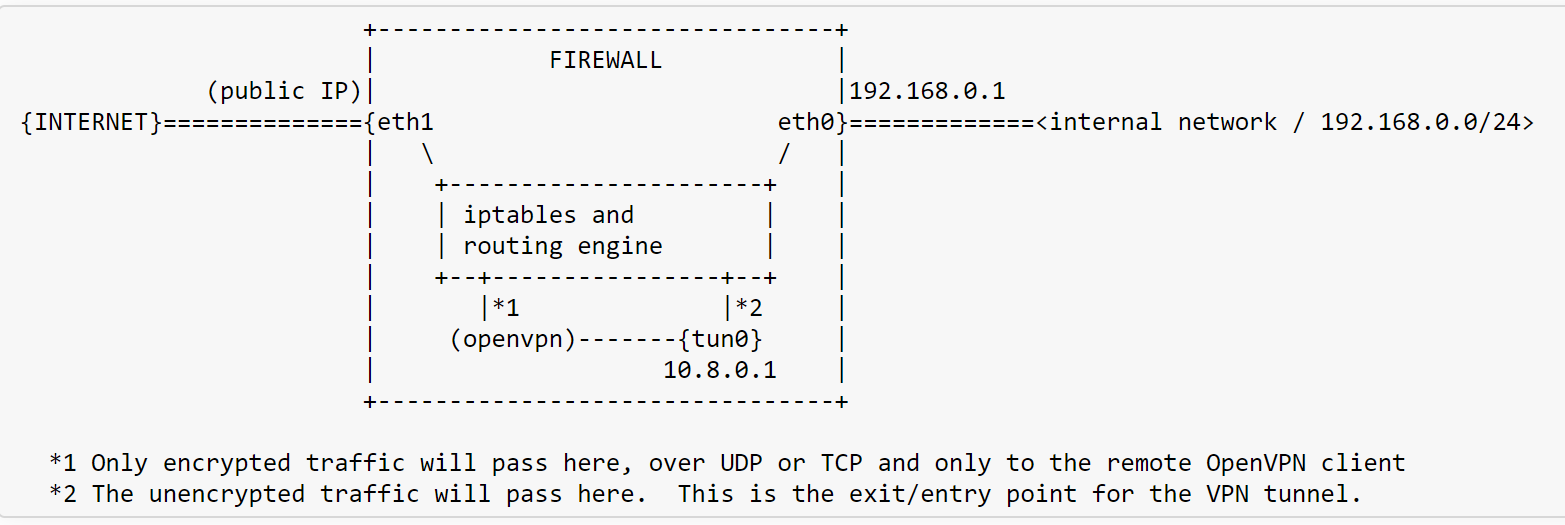
\includegraphics[width=1\textwidth]{images/openvpn_routing_setup.PNG}

	When a packet arrives at the ``eth1'' interface, OpenVPN picks it up, decrypts, and sends the data to the tun0 interface. The ``iptables'' and the routing engine filter and masquerade the packet and send it to eth0, where it becomes available to the final receiver.\\
	In the other direction, when the packet arrives at ``eth0'' interface, ``iptables'' and the routing engine apply their rules to filter and masquerade, and then they forward it to ``tun0'' interface. Thus, OpenVPN picks it up, encrypts the data, and sends it to the public ``eth1'' interface.\\
	In our scenario, the network configuration is slightly different and does not include an internal interface network. As the schema below describes, OpenVPN sends the traffic coming from ``tun0'' to the public interface eth0 on a specific port. The client application listens on that port, and the OpenVPN client decrypts the received data.\\

	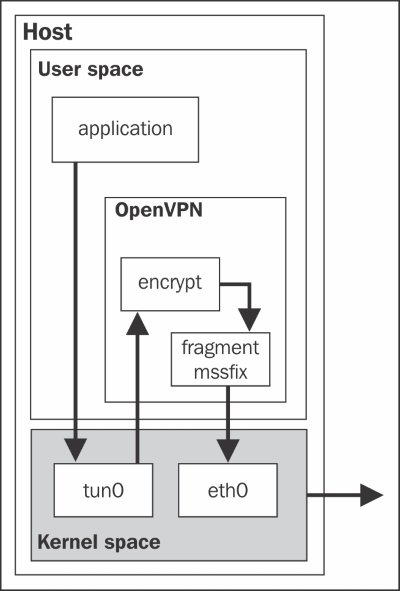
\includegraphics{images/openvpn_tun_interface.jpg}

	IMAGE TO EDIT AS BEFORE DESCRIBED\\

	\subsubsection{Start a node}
	There are two ways to start a Mysterium node. The first one is using the Docker image: Docker is a platform that uses the OS virtualization to deliver software in packages called containers. The image contains all the specifics that the application requires to be executed.\\
	From the software image, Docker creates as many containers as we instantiate, and they are the virtualized software we will use.  We can think of the software image as the house project and the software container as the real house construction. As the house construction can have personalizations, either the container is set up passing parameters to customize the network, the storage, or other settings such as the resources allocated by Docker to the single container.\\
	With the following command, we pull the image of the Mysterium node to the Docker platform:
	\begin{verbatim}
		docker pull mysteriumnetwork/myst
	\end{verbatim}
	
	Then, we create the container using:\\

	\begin{verbatim}
		sudo docker run --cap-add NET_ADMIN --net host --name myst -d mysteriumnetwork/myst service --agreed-terms-and-conditions --openvpn.port 1194
	\end{verbatim}

	The parameters specify, from left to right:
	\begin{enumerate}
		\item to add the network capability to the operative system, which is Linux,
		\item to connect the container to the net,
		\item to name the container ``myst'',
		\item to run the container in background mode and detach it from the shell.
	\end{enumerate}

	The remaining values are passed to the Mysterium software. The ``service'' value means Mysterium node starts as a node, thus a service provider, instead of a client, the next one is to agree on the terms and conditions, and the last one is to set up the OpenVPN port.\\
	When the container is up and running, we can check the logs using:

	\begin{verbatim}
		sudo docker logs -f myst
	\end{verbatim}
	
	We can find relevant details reading the log, such as the identity registration and the node proposal:
	\begin{verbatim}
		...
		[Mysterium.api] Identity registered: 0x4cd126119cd14e38c90e34dd8b6e0e2174b71123
		[Mysterium.api] Proposal pinged for node: 0x4cd126119cd14e38c90e34dd8b6e0e2174b71123
		...
	\end{verbatim}

	The identity registration is the unique ID assigned from the network to the node. With this ID, it is possible to discover it, its connection details, and transaction history on the Mysterium Network website.\\
	
	
	The second way to install the Mysterium node is using the Debian package. To manage its execution, we use the ``systemctl'', a management tool for controlling the init system:\\
	We run 

	\begin{verbatim}
		sudo systemctl daemon-reload
	\end{verbatim}

	to reload the daemon after the changes to the node settings, and 
	
	\begin{verbatim}
		sudo systemctl restart mysterium-node
	\end{verbatim}
	
	to reload the node.\\

	If the node is up and running, it exposes a web interface on the localhost available at port 4449, where it is possible to control the service status and see connection statistics.
	
	\subsubsection{Connect to a node}

	When the node works, the simplest way is to use the mobile or desktop client applications that provide a graphical interface to choose the server node and establish the connection. In a few seconds, the Mysterium network creates the connection record in the blockchain, initializes the connection and, then, the VPN takes place.\\

	Another way to connect to the service provider is using the command-line interface the node as a client exposes. Referring to the node installed by the Debian package, the command to run the node and control it is:\\
	
	\begin{verbatim}
		myst cli
	\end{verbatim}

	We then enter in a view where we can perform the operations on the node that regard the identity management, the connection creation and the status diagnostic.

	\subsubsection{Iptables}

	The ``iptables'' is a framework to manage the network decisions. It is based on the ``Netfilter'' kernel component, which exposes a set of hooks that are triggered at specific points of the network stack. Every packet that enters the networking system will trigger these hooks as it proceeds through the stack so all the programs that register with these hooks can interact with the traffic.\\
	Five different hooks correspond to different points of the stack:\\

	\begin{itemize}
		\item \lstinline{NF_IP_PRE_ROUTING}
		\item \lstinline{NF_IP_LOCAL_IN}
		\item \lstinline{NF_IP_FORWARD}
		\item \lstinline{NF_IP_LOCAL_OUT}
		\item \lstinline{NF_IP_POST_ROUTING}
	\end{itemize}

	IMAGE OF THE POINTS IN THE FLOW WHERE THE HOOKS ARE
	
	Iptables is mainly used as a firewall which organizes its rule in tables and chains. The tables classify the rules according to the type of decision that regards the packet.\\
	The available tables are the filter table, the NAT table, the Mangle table, the Raw table, and the Security table.\\
	The chains correspond to the available hooks, therefore iptbales has the \textbf{prerouting}, \textbf{input}, \textbf{forward}, \textbf{output}, and \textbf{postrouting} chains.\\
	The following table explains the triggering logic and execution precedence.\\

	\begin{tabular}{|l|c|c|c|c|c|}
	\textbf{\begin{tabular}[c]{@{}l@{}}Chains\\ Tables\end{tabular}} & \rotatebox[origin=c]{90}{\textbf{PREROUTING}}    & \rotatebox[origin=c]{90}{\textbf{INPUT}}         & \rotatebox[origin=c]{90}{\textbf{FORWARD}}       & \rotatebox[origin=c]{90}{\textbf{OUTPUT}}        & \rotatebox[origin=c]{90}{\textbf{POSTROUTING}}   \\\hline
	\textit{ruoting decision} & & & & X & \\\hline
	\textbf{raw} & X & & & X & \\ \hline
	\textit{connection tracking enabled} & X & & & X & \\\hline
	\textbf{mangle} & X & X & X & X & X \\\hline
	\textbf{DNAT (NAT)} & X & & & X & \\ \hline
	\textit{routing decision} & X & & & X & \\ \hline
	\textbf{filter} & & X & X & X & \\ \hline
	\textbf{security} & & X & X & X & \\ \hline
	\textbf{SNAT (NAT)} & & X & & & X
	\end{tabular}

	The packet triggers the hooks from the first row going down to the bottom of the table. It enters the chain depending on the routing decisions that are made based on its direction, incoming or outgoing, and whether the filtering rule accepts the packet.\\

	The chain traversal order is the following:
	\begin{itemize}
		\item Incoming packets destined for the local system: PREROUTING - INPUT
		\item Incoming packets destined to another host: PREROUTING - FORWARD - POSTROUTING
		\item Locally generated packets: OUTPUT - POSTROUTING
	\end{itemize}
	
	Every chain is a list of rules. Every packet is checked against each rule and, if the matching component checks, iptables executes an action.\\
	The rule can match the packet depending on the protocol type, the source or destination address, or packet, among other criteria.\\
	The action called target, which is triggered if the rule matches, can be of terminating or non-terminating type.\\
	The terminating type target causes the packet to exit the chain after a verdict that can be to allow or to drop the packet. The non-terminating type target causes the packet to continue its evaluation in the chain. There can be any number of non-terminating targets before a terminating one.\\
	A very used non-terminating target is the jump action: a rule can decide to jump a packet into another chain, and when that chain finishes the rules check, the execution comes back to the previous chain. This way is useful to organize the rules in chains based on their purposes.\\

	LITTLE IMAGE OF CHAIN JUMP ACTION

	With ``iptables'', it is possible to build firewalls and control systems to manage the computer network efficiently.


	\subsection{Design vulnerabilities}

	Mysterium is a complex system that integrates components of different types. The distinct nature of these components and their conjunction opens to new vulnerabilities scenarios where the focus is on the system overall and how the elements dialog each other.\\
	In the following chapter, we provide considerations on the Mysterium Network system concerning its components and their integration. In order to do this, we had to assumed some components behaviours and their impact on the system because Mysterium does not implement them yet, at this time. Indeed, Mysterium project is under development, which plans to have a fully decentralized network in 2021. 

	We classify the several aspects that, on a project like Mysterium, must be considered to evaluate its design vulnerabilities based on:
	\begin{itemize}
		\item the position in the network: starting, middle or endpoint point;
		\item the step of the flow: the service proposals, the promise issuing, the transaction closing, and other steps;
		\item the operations on the passing data: sniffing, filtering or crafting the data;
		\item side channels attack and other particular scenarios.
	\end{itemize}
	
	\subsubsection{The position in the network}

	In the simplest configuration, the network includes a starting point that is the service consumer node and an endpoint, which is the service provider node. The VPN tunnel connects the two nodes and encrypts their traffic. The service node, as previously described, is the consumer's exit point to the internet.\\
	We consider secure the traffic passing through the VPN tunnel because it is encrypted, not secure otherwise, that is from the provider to the internet.\\

	SIMPLE NETWORK CONFIGURATION WITH AN EXIT NODE\\

	The exit nodes connect two areas with two different security levels: for this reason, it is sensitive by default and without specific precautions can be the weak link of the system.\\
	The Tor network has a similar problem. Tor stands for The Onion Router, and it is a network of peers where the user's encrypted traffic is sent into, and it bounces multiple times before getting an exit node from where, finally, it reaches the external resource.\\
	The traffic is encrypted for each bouncing, except the last one, where it must be in clear to connect to the internet resource. The end node's role is to decouple the encrypted network from clear internet, and this makes it so valuable. If an exit node is malicious, it can potentially understand all the data passing through it and going to the internet resource.\\
	Dan Egerstad is a Swedish computer security consultant. He intercepted thousands of diplomatic emails setting up malicious exit nodes around the world and sniffing the connection between them and the clear internet \cite{exitnodeTOR}.\\
	To discover malicious nodes in the Tor network, another Swedish researcher built up a website with a login and a system to count the login attempts. Then, he used multiple Tor paths with different exit nodes to access the page. The system counted more login attempts that the researcher have done: this means some exit nodes sniffed the connections, caught the username and password, and tried to login by themselves \cite{exitnodeTOR2}.\\
	In both cases, the use of HTTP instead of HTTPS, or of other unencrypted protocols, has been necessary, but the research aim was to demonstrate the exit nodes' critical role because there still are many protocols and applications that do not use encryption for their traffic.\\
	The conclusion is that Tor's end nodes are the weak link of the system when the users use it as an end-to-end encryption network, rather than an anonymization network, as well as Mysterium Network end nodes.\\
	For this reason, many of the conceptual vulnerabilities held by the exit node of Tor can be applied to a Mysterium Network exit node. But we want to point out a difference between Tor and Mysterium networks: the type of target users of the two projects.\\
	The Tor's users use it to accomplish specific online activities where the identity obfuscation is mandatory. For the rest of the actions, Tor is not efficient, can be blocked by ISP and, in some countries, is even banned.\\
	The Mysterium Network users, instead, use it for a broader range of online activities, and we can assume the use with a persistent connection to the VPN network with almost no impact on the user's system. In this direction, the implementation of the mobile app is crucial: smartphones are becoming the first device from where people access the internet and the capability to have a device connected all the time with the VPN network provides a security level not yet implemented for consumer uses.\\
	This scenario, however, introduces move vulnerabilities simply because the network is used for more activities, and many protocols and applications still use unencrypted communication.\\
	
	
	Figure X describes the network configuration of a Mysterium end node.\\
	The provider manages all the traffic from the VPN tunnel, both incoming and outgoing and because it has not the VPN encryption, he can potentially perform all the manipulation he wants. We will discuss further this scenario analyzing the technical solutions and providing a practical example to exploit in chapter X.\\
	\textit{If we ask someone to look at a photo for us and tell us to describe its content, he must, of course, understand the meaning, can change a little detail, or even tells someone else the content of the picture.}\\
	An improved configuration implies one or more middle points between the consumer and the provider. Those points are called hops, and they act similarly to the provider node since they forward the traffic.\\
	Mysterium did not implement those hops in the network yet. Therefore we make a hypothesis on its possible implementation.\\
	As well as for the provider nodes, we can suppose there is a distributed list of the forwarder nodes. When the consumer chooses the provider, and they agree to issue a payment promise, the network picks a node from that list to place it as the hop. The middle node receives a new VPN connection from the consumer and creates a new VPN connection to the provider. He technically builds and manages two different VPN tunnels: it takes encrypted data from one side, decrypts them, and encrypts again to send on the other one.\\
	The scenario is similar to the end node because the middle node holds unencrypted data in the forwarding action.\\
	The following picture well describes the situation with even more than one hop. We would have a segmented connection, called multihop connection, between the ends, where all the hops can perform unwanted operations on the traffic.\\

	IMAGE OF MULTIHOP CONNECTION.\\

	Mandatory would be an additional encryption layer end to end, over the VPN encryption between each node, that the consumer and provider have to manage. This second encryption solves the multihop data exposing because the middle nodes would manage only data encrypted by the second layer. The cons are that it increases the computational load.\\
	The vulnerabilities, in this scenario, are restricted to all the operations that concern the traffic shape, with no abilities to understand it. These actions hit the quality of service, a class of attacks that aim to lower or even block the service.\\
	Many traffic shapes operations can be performed on a connection: the simplest and the fastest is on the traffic speed, and it does not need to understand the content at all.\\
	A demonstration of how a middle node can slow down the data speed that it forwards, is using a Linux package called \tag{tc} \cite{tc}. It stands for Traffic Control, and it is created and used for service quality analysis.\\
	With the following command, we instruct the network manager to apply a delay of 500 milliseconds for every packet sent to the interface \tag{eth0}.\\
	
	\begin{lstlisting}
		sudo tc qdisc add dev eth0 root netem delay 500ms
	\end{lstlisting}
	
	Here is what each option means:
	\begin{itemize}
		\item qdisc: modify the scheduler (also known as queuing discipline)
		\item add: add a new rule
		\item dev eth0: rules will be applied on device eth0
		\item root: modify the outbound traffic scheduler (aka known as the egress qdisc)
		\item netem: use the network emulator to emulate a WAN property
		\item delay: the network property that is modified
		\item 500ms: introduce delay of 500 ms
	\end{itemize}

	With the following command, we delete the delay rule.\\

	\begin{lstlisting}[frame=single]
		sudo tc qdisc del dev eth0 root netem
	\end{lstlisting}

	In this simple way, the traffic speed between the consumer and the provider has a poor quality because one or more middle points are performing this slowing down the operation. From the consumer side, the poor connection is a quality agreement breach, and it affects the service provider's reputation. Since the provider can detect the slow speed, he can suppose it is a packet path issue and can propose to the network to change one or more middle nodes. 

	\subsubsection{The flow steps}
	The first and easiest idea to implement to use the system maliciously has already been presented before: the attacker is the consumer, he creates an account in the Mysterium Network, has a positive balance to the cryptocurrency wallet, and look for a service proposal. They agree on the service cost and issue a payment promise. If the user does not respect the promise...
	TODO\\

	\subsubsection{Operations on the passing data}

	In this section we analyze the different operation an end node can perform, based on the fact it manages traffic outside the VPN tunnel.\\
	The traffic outside the tunnel is not encrypted by the VPN, but this does not necessarily mean it is not encrypted by itself. Some protocols encrypt data by design. Others do not encrypt or have different structure levels where the lowest have no encryption at all and can be modified.\\ Based on this consideration, the operations that a node can potentially do on the passing data can be grouped in sniffing, filtering, and crafting.\\
	The first step to manipulate the data is to catch it, and we want to show an example of how-to-do. After starting a Mysterium Node on our test server and then establish the connection to it using a Mysterium client, we use \tag{tcpdump} to dump the traffic of the network. For the example purpose, we get an online resource hosted on a different server and available using the HTTP protocol, so that the dumped traffic is in clear.\\
	Our example provides an HTTP request to the host www.jafed.xyz with the method GET to obtain a file named test.txt with the content the string "cool, you got me sir!".\\
	The request is executed using curl, a command-line tool for transferring data using various protocols.\\

	\begin{lstlisting}[frame=single]
		curl www.jafed.xyz/test.txt
	\end{lstlisting}
	
	With the following command, instead, we capture the request specifying the output format defined by \lstinline{-v} \lstinline{-n} \lstinline{-l}, then we pipe it to the \lstinline{egrep} command to parse the string and return an easy-to-read text:\\
	
	\begin{lstlisting}[frame=single]
		sudo tcpdump -v -n -l | egrep -i "POST /|GET /|Host:"
	\end{lstlisting}

	A slice of output is\\
	
	\begin{lstlisting}[frame=single]
		GET /test.txt HTTP/1.1
        Host: www.jafed.xyz
	\end{lstlisting}

	that shows we caught the HTTP request.
	
	We use Wireshark to analyze the content, a powerful graphical application for network usages. It supports the pcapng file extension that tcpdump uses to save the data.\\
	We print the captured result filtered of the packets of our interest:\\
	
	\begin{lstlisting}[frame=single]
		GET /test.txt HTTP/1.1
		Host: www.jafed.xyz
		User-Agent: curl/7.58.0
		Accept: */*

		HTTP/1.1 200 OK
		Date: Sun, 09 Feb 2020 16:59:45 GMT
		Server: Apache
		Upgrade: h2,h2c
		Connection: Upgrade
		Last-Modified: Thu, 06 Feb 2020 21:49:33 GMT
		ETag: "1ae1c77-15-59def3f9b28fd"
		Accept-Ranges: bytes
		Content-Length: 21
		Content-Type: text/plain

		cool, you got me sir!
	\end{lstlisting}

	

	\subsubsection{Side channels attack and particular scenarios}
	In this section, we discuss the possible scenarios that do not directly regard attacks on specific components, but more on how these harmless operations in Mysterium Network lead to vulnerabilities.\\
	In Mysterium Network, the billing method is per the amount of transferred data or per time. Considering the first method, if the exit node is able to higher the volume of the traffic to the consumer, it means the exit node earns money without providing an equal service. A well-designed attack can perform the traffic shaping hiding the increase of traffic volume with network inefficiency.\\
	In the "tcp/udp" subsection in the Craftberry tool description, we implemented an attack that uses this technic to make multiple copies of the packets using tcp and udp protocols with no content understanding. A more refined attack would be modifying the packet specifically for the protocol, forcing the error in the communication so that the protocol corrects it. In this document, we did not focus on those particular cases which are deeply protocol dependent, but the modification aims to increase the transmitted data because the bill is calculated on that.\\
	
	VLAN tag attack when the client is into an enterprise network. The attack crosses the firewall of the infrastructure.

	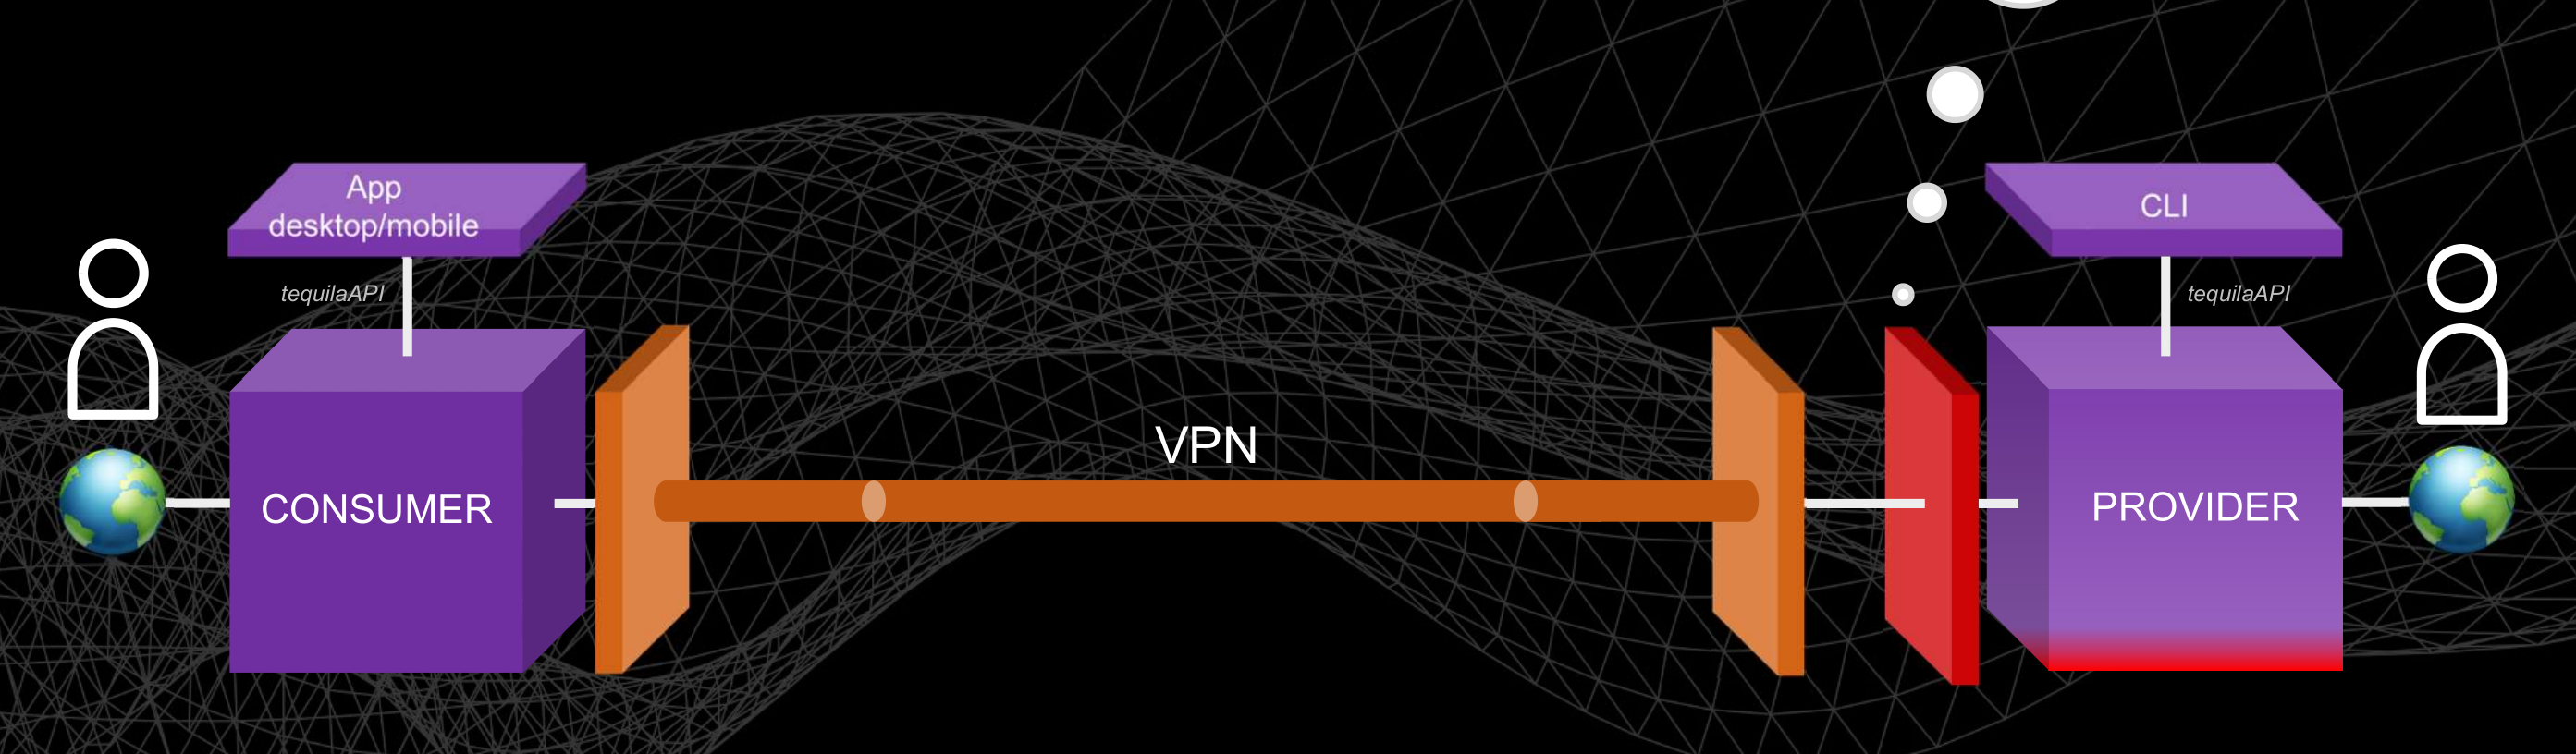
\includegraphics[width=\linewidth]{images/client_server_vpn_connection.png}

	\section{Craftberry}

	\subsection{The idea}
	Craftberry is a proof of concept tool to demonstrate how a node can sniff, filter and craft the outgoing traffic from an exit node of the Mysterium Network.\\
	It is an application that runs via the command-line interface. It catches the incoming or outgoing packets in line with the packet flow, and it executes different actions accurately implemented to cover many attack and defense cases.\\
	The software is entirely written in C and C++. It uses the \tag{nfqueue} extension to move the packet from the kernel space to the user space, where it is crafted and sent back to the kernel space to continue the network traversal. The application uses the PcapPlusPlus library to parse the packet, build its layers, and modify the content.\\
	The application sets up the iptables rules to redirect the packets. These rules follow the Craftberry action passed via CLI.\\
	
	We propose part of the output provided by the application when the help command is used:
	\begin{itemize}
		\item \lstinline{-a}: Use the specified action
		\item  \lstinline{-i}: Use the specified interface, tun0 by default. Can be interface name (e.g. eth0) or interface IPv4 address
		\item  \lstinline{-t}: Use the specified timeout in seconds, if not defined it runs until some external signals stop the execution (e.g. ctrl+c)
		\item  \lstinline{-l}: Write all the crafted and generated traffic into a \lstinline{pcapng file} having name passed by parameter or, if the parameter is equal to 'default', the name is \lstinline{out_<epoch_ms>.pcapng}
		\item  \lstinline{-d}: Direction filtering by and perform the crafting {IN, OUT}, default = IN
		\item  \lstinline{-v}: Shows verbose debug application logs
		\item  \lstinline{-h}: Displays this help message and exits
	\end{itemize}
		
	The parameter set by \tag{-a} defines the action Craftberry has to perform when it catches a packet. We divide the operations into two categories: attack or defense. The attack operations are the most interesting for this research, but we also implemented a defense solution that protects the passing traffic encrypting the packet content.\\
	The attacks differ on which ISO-OSI layer the packet is crafted.\\

	IMAGE OF THE ISO OSI LAYERS MODEL\\
	
	The attack actions categorized by layer are:
	\begin{itemize}
		\item Layer 2: VLanDoubleTagging
		\item Layer 3: IP, icmp
		\item Layer 4: tcp/udp
		\item Layer 5 and above: HTTP, DNS, NTP
	\end{itemize}
	
	side attacks:\\
	- auditin/collezione dei dati sniffati, inviati ad un server esterno per collezionamento, statistiche, vendita a terzi.
	- trojan all'interno di craftberry, per botnet. (approfondire aspetto che se il sw di attacco diventa popolare, può essere lui stesso veicolo di malware, quindi attacco l' attaccante)

	The defense action is at layer 4. It encrypts the payload of the packets with \tag{ChaCha20} algorithm, a \tag{Salsa20} modification published in 2008. It is a particularly efficient stream cipher.\\

	\subsection{nfqueue extension}
	NFQUEUE is a kernel and user mode module for managing network packets in iptables. It allows writing \tag{Netfilter} target modules in userspace. This module is an application that is called by \tag{nfqueue} hooks. In the program, the hooks are bonded to a function that is called when the iptables match a rule.\\
	The function gets the queue details and the packet payload, it can craft the packet, and then send a verdict to the iptables module. 

	FLOW OF THE PACKET (CATCHING, CRAFTING AND THEN VERDICTING IT)

	\subsection{PcapPlusPlus}
	It is a multiplatform C++ library for capturing, parsing, and crafting of network packets. As major features, there are that it is designed to be efficient, powerful, and easy to use. It is a wrapper for the most famous packet processing engines making easy decoding and forging a large variety of network protocols.
 
	\subsection{Actions}
	\subsubsection{VLan double tagging}
	use the double tagging attack method on cisco routers


	\subsubsection{IP}
	The IP packet contains information of the source and the destination IP address. The goal of this attack is to change the destination address to redirect the packet somewhere else.\\
	

	\subsubsection{icmp}

	\subsubsection{tcp/udp}
	
	The context of the attack supposes that the communication is encrypted supplementary to the VPN encryption. It is provided by end-to-end encryption between the Mysterium client and the server it is communicating with, and not the exit node. Therefore, the exit node cannot then perform any content understanding, and only actions on the entire packet can be done, as described in the Design vulnerabilities chapter.\\
	The attack accomplishes a simple copy of the packet: when the provider receives packets from the internet, it sends \tag{n} times a copy of the captured packet to the consumer.\\
	The implementation is as simple as significant: with this method, with no content understanding, the passing data are more than the necessary, and the service consumer is affected.\\

	\bigbreak
	
	We have implemented a demonstrative example of this attack using the protocols \lstinline{tcp} and \lstinline{udp}.\\

	The code in the main function is the following:\\
	\begin{lstlisting}[frame=single]
		if (conf->method.compare("ICMPMULTIPLY") == 0 && Action::Icmp::isProto(inPacket)) {
			Action::Tcp *action = new Action::Tcp(n);
			action->multiply(inPacket->getRawPacket());
			return verdict_accept(qh, ntohl(ph->packet_id), inPacket);
		}
	\end{lstlisting}

	The multiply method is implemented as follows:
	\begin{lstlisting}[frame=single]
		void multiply(RawPacket *inPacket) {
			for (int i = 0; i < this->n; i++) {
				sendPkt(inPacket);
			}
		}
	\end{lstlisting}

	The \lstinline{n} parameter is a TCP class field. 

	\subsubsection{DNS robber}

	Malicious DNS redirect: https://securitytrails.com/blog/dns-hijacking\\

	This attack can be used for phishing or data collecting attacks. The first one attempts to obtain sensitive information by disguising oneself as a trustworthy entity in an electronic communication. In our case, the idea is to redirect the requested page to a fake page which matches the look and feel of the legitimate site.\\
	The second one, instead, uses the change of the URL to redirect the request on a website to record it.

	\subsubsection{HTTP}

	Hypertext Transfer Protocol is an application-layer protocol for transmitting hypermedia documents, and it is the standard in the client-server architectures. The HTTP protocol is stateless, meaning that the server does not keep any state between two requests.\\
	This protocol is perfect for implementing an attack and for demonstrating how a node can maliciously and heavily modify the content of a packet. Our goal is to intercept the response of a HTTP answer, detect if the payload is an image and then substitute it with another one. We need to clarify that the HTTP response content can be splitted over many tcp packets, if it is larger than the maximum tcp packet size. Craftberry captures tcp packets, but does not perform tcp reassembly. Therefore, for our demonstration purpose, it can operate the image substitution only for images contained in a single tcp frame.

	
	\begin{itemize}
		\item http://linux-training.be/networking/ch14.html
	\end{itemize}

	\begin{verbatim}
		http://unixwiz.net/techtips/gnu-c-attributes.html
		https://gcc.gnu.org/onlinedocs/gcc-4.0.2/gcc/Type-Attributes.html
		https://groups.google.com/forum/#!msg/pcapplusplus-support/e7rN93LfTSg/MFnVEKCNCAAJ
		https://byt3bl33d3r.github.io/using-nfqueue-with-python-the-right-way.html
		
	\end{verbatim}
			
	\subsection{Tests}
		???
	\subsection{Design solutions for malicious context}
		\subsubsection{comparing data}
		invia la richiesta a due nodi e le confronta (essenziale possibilità di connessione a due nodi in contemporanea: due o più container docker mappati su porte diverse con uno script che invia la richiesta a più container e confronta le risposte)

		\subsubsection{comparing hashes}
		come precedente ma con la gestione degli hash invece che di tutto il dato
		
\section{Conclusions}
	\subsection{Future development}
	\subsection{Considerations}

	The use of Mysterium Network like an end-to-end encryption tool: https://nakedsecurity.sophos.com/2015/06/25/can-you-trust-tors-exit-nodes/
	Here there is a helpful consideration of how critical is an exit point for TOR.

	\pagebreak

	\bibliographystyle{plain}
	\begin{thebibliography}{1}
		\bibitem{HTTPS}
			HTTP Over TLS - RFC
			https://tools.ietf.org/html/rfc2818
		\bibitem{VPNRFC}
			A Framework for IP Based Virtual Private Networks - RFC
			https://tools.ietf.org/html/rfc2764
		\bibitem{tc}
			Traffic Control
			https://jvns.ca/blog/2017/04/01/slow-down-your-internet-with-tc/
		\bibitem{exitnodeTOR}
			exit nodes of TOR network
			https://www.wired.com/2007/09/rogue-nodes-turn-tor-anonymizer-into-eavesdroppers-paradise/?currentPage=all
		\bibitem{exitnodeTOR2}
			malicious TOR exit nodes
			https://www.makeuseof.com/tag/priority-wretched-hive-scum-villainy-5-ways-stay-safe-bad-tor-exit-nodes/
	\end{thebibliography}
		
	\pagebreak
	
	%%	{\Large Valutazione di un nuovo utente della rete}
	\paragraph{Contesto}
	Rete VPN decentralizzata attiva e con connessione multi-hop tra una generica coppia Agent-Client.
	
	\paragraph{Problema 1: identificare gli Agent in posizione endnode che inviano contenuto non originale}
	In una rete VPN decentralizzata gli Agent endnode hanno il compito di recuperare una risorsa web e restituirla al Client attraverso la rete VPN instaurata. L'Agent, che quindi ha accesso intrinseco al dato ottenuto, cifrato o meno, può modificarlo prima di inviarlo al Client. Questa operazione può avere scopi malevoli, tra cui quello del guadagno economico. In possibile scenario, in questo contesto, è quello che vede l'incremento della grandezza del pacchetto da Agent a Client al fine di maggiorare i consumi della banda stabilita nel contratto iniziale di fornitura del servizio.
	
	\paragraph{Problema 2: scoraggiare abusi della rete}
	Per scoraggiare abusi della rete si utilizza una \textit{prova di lavoro} (Proof of Work) per attestare che il nuovo utente della rete ha speso delle risorse al fine di guadagnare reputazione nel contesto distruibuito.\\
	La reputazione iniziale, all'ingresso della rete distribuita, ha valore zero.
	
	\paragraph{Soluzione problema 1}
	\begin{itemize}
		\item Dati civetta: è richiesta dal Client all'Agent, con frequenza variabile, una risorsa dal valore noto al Client per la verifica di integrità. Se il test risulta negativo si ipotizza la modifica della risorsa da parte dell'Agent.
		\item Dati duplicati: il Client si connette a due Agent diversi e chiede ad entrambi la risorsa desiderata, alla ricezione si comparano per la verifica di integrità. Se il test risulta negativo si ipotizza la modifica della risorsa da parte di uno dei due Agent.\\
		\textbf{Aspetti negativi:} questa soluzione non è applicabile in caso di connessioni con la risorsa che prevedono \textit{stati}.(??)
		\item Hash Dato: il Client si connette ad un Agent al quale chiede una risorsa e successivamente chiede ad un altro Agent l'hash della risorsa stessa. Il Client effettua quindi un hash (stessa funzione hash) della risorsa ottenuta dall'Agent e la compara con l'hash ottenuto dal secondo Agent. Ulteriore implementazione può essere effettuata richiedendo a più agent l'hash della risorsa.\\
		Se il test risulta negativo si ipotizza la modifica della risorsa da parte del primo Agent.\\
		\textbf{Aspetti negativi:} questa soluzione non è applicabile in caso di connessioni con la risorsa che prevedono \textit{stati}.\\
		\textbf{Caso d'uso:} si reputa questo metodo adatto a verificare un Agent al suo primo ingresso nella rete in quanto non è spesso adatto per l'aspetto negativo sopra descritto.		
	\end{itemize}
	
	\paragraph{Soluzione problema 2}
	L'originalità della soluzione proposta è l'operazione di Proof of Work da far compiere al nuovo utente. Si propone come prova di lavoro che l'utente, prima di entrare attivamente a far parte della rete o durante la sua partecipazione, consumi della banda internet.\\
	La Proof of Work, quindi, consiste nello sfruttare la sua banda internet per ottenere una risorsa internet, sulla quale viene verificata l'integrità, come descritto nella soluzione \textit{Dato Hash} proposta nella soluzione al problema 1.\\ 
	Più specificatamente, nel caso d'uso si identificano un Agent A, un Client C ed un nuovo utente X che vuole entrare nella rete e deve dimostrare \textit{la prova di lavoro}.\\
	La situazione iniziale prevede una connessione tra A e C. Per verificare che A fornisca dato $d^A$ originale, C richiede a X di ottenere lo stesso dato $d^X$ e di eseguirne la funzione hash così da ottenere  $H(d^X)=h_1$. $h_1$ sarà restituito a C che ha già effettuato la stessa funzione hash su $d^A$ proveniente da A ed ha ottenuto $H(d^A) = h_2$.\\
	Il test di integrità verifica che $h_1 = h_2$.\\
	Se il test ha successo si ha certezza che:
	\begin{enumerate}
		\item il nuovo utente X ha eseguito correttamente la proof of work 
		\item A ha fornito a C un dato originale, a meno che sia A che X applichino le stesse modifiche al dato prima di effettuarne la funzione hash.\\Questa vincolo è da verificare.
	\end{enumerate}
	
	\paragraph{Considerazioni}
	In un contesto di rete distribuita si possono ipotizzare $n$ attori nel ruolo di X e $n$ test di integrità che C effettua per verificare l'integrità del dato ottenuto da A. \textit{riferimento al consenso BFT}\\
	Il risultato dei test condiziona la reputazione di ogni attore nel ruolo di $X$.\\
	Si può ipotizzare l'applicazione della soluzione $m$ volte, tante quante sono le entità per cui effettuare la proof of work, e considere vincoli come tempo $t$ minimo di esecuzione della proof of work o la quantità minima di dati $q$ che $X$ deve ottenere su cui applicare la funzione hash.\\
	
	
	Considerando una costo ipotetico $c$ associato al consumo di una quantità $q$ di dati per un'unità di tempo $t$ si può impostare una soglia $S = c*q*t$ superata la quale la proof of work si può considerare eseguita.\\
	L'ultima affermazione garantisce l'asimmetria della proof of work (??). (che è: hash difficile da calcolare perchè spendo risorsa di tempo e di banda e facile da verificare dal client perchè effettuo un semplice confronto di un hash)(vedere https://it.wikipedia.org/wiki/Hashcash per similitudini sulla variabile del tempo)\\
	
	
	La reputazione di ogni entità all'interno della rete, sia Agent che Client, subisce una variazione in quanto ciascun esito delle proof of work viene registrata nella blockchain e questo consente di avere una classifica di affidabilità delle entità quasi in tempo reale.\\
	

	

\end{document}